%http://neutrino.fnal.gov/events/summer_lecture_series/slides2016/Zarko-Pavlovic-Sources.pdf
%http://microboone-docdb.fnal.gov:8080/cgi-bin/RetrieveFile?docid=5787&filename=bnb-flux-microboone.pdf&version=4
The purpose of this chapter is to describe how neutrinos are produced in the Booster Neutrino Beam-line (BNB) at the Fermi National Accelerator Laboratory. An understanding of how these neutrinos are produced and their flux through the MicroBooNE detector is necessary to properly interpret the results of the low energy excess analysis and kaon production analysis, described in Chapters \ref{sec:LEEhistory} and \ref{sec:LEEsensitivity}. In describing the neutrino production techniques, the reader will be introduced to the sources of systematic uncertainties associated with the neutrino production, both in terms of how they arise, and their magnitude. 

\section{The Booster Neutrino Beam}\label{beam_descript_section}
The Boost Neutrino Beam-line (BNB) collides protons at 8.89 GeV/c momentum from the Fermilab Booster synchrotron with a beryllium target to produce a high flux of neutrinos. The layout of the BNB is shown in Figure \ref{BNB_layout_schematic}~\cite{MBFluxPaper}, and the relevant steps of the neutrino production process will be described in the following sections.

\begin{figure}[ht!]
\centering
	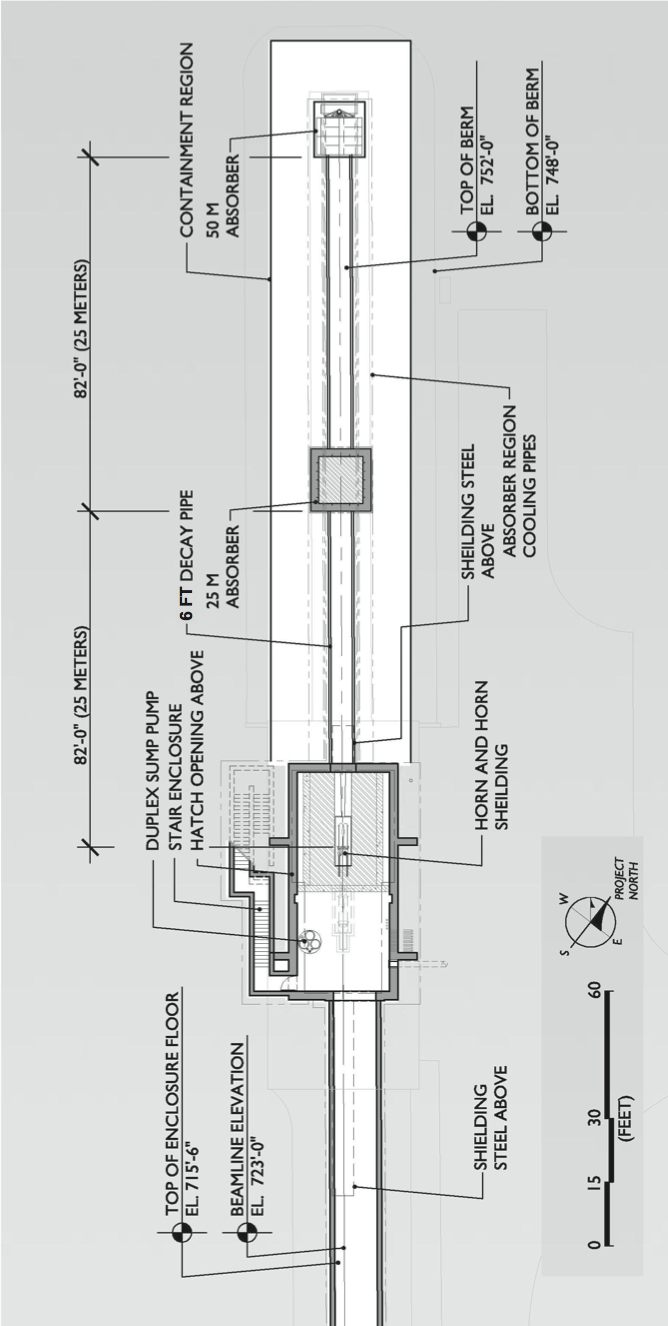
\includegraphics[width=0.5\textwidth]{Figures/BNB_layout_schematic.png} \\
\caption{\textit{Overall layout of the BNB. The primary proton beam, extracted from the Booster, enters the target hall from the left. Upon exiting the target hall, particles encounter a 50-meter-long decay region, terminating in the beam stop on the right.}}\label{BNB_layout_schematic}
\end{figure}

\subsection{Primary Proton Beam}
The protons originate from $H_2$ gas molecules converted to $H^-$ ions via a Cockroft-Walton generator, and are initially accelerated to approximately 1 MeV kinetic energy. These ions are subjected to a linear accelerator using alternating electromagnetic fields to increase their energy to about 400 MeV. Passing through a carbon foil removes electrons, and the bare protons enter the Booster synchrotron where they are accelerated up to 8.89 GeV/c momentum. The protons are bunched in ``beam spills'' containing roughly $4\times10^{12}$ protons spaced throughout a 1.6 $\mu s$ time window per spill. The protons are then directed towards a thick beryllium target.\\

The absolute number of protons directed on target (POT) is measured by two toroids upstream of the target which are part of a larger beam monitoring system. The error on the POT is on the order of 2\%. Additional beam characteristics are monitored by beam position monitors (BPMs), a multi-wire chamber, and a resistive wall monitor (RWM) which together measure beam intensity, timing, width, position, and direction.

\subsection{Proton Target and Focusing Horn}
The beryllium target is 71.1 cm long, which corresponds to 1.7 proton interaction lengths, and is 0.51 cm in radius. Beryllium is chosen as the proton target because its relatively low Z (4) minimizes radiative losses from the protons before their p-Be interactions which produce secondary mesons ($\pi^\pm$, $K^\pm$, $K^0_L$).\\

The beryllium target is located within a larger focusing electromagnet, referred to as the horn. A schematic drawing of the horn is shown in Figure \ref{BNB_horn_schematic}. The horn is an aluminum alloy pulsed toroidal electromagnet. The pulsed current has a peak at 170 kA and a time-width of 143 $\mu s$, coincident with the proton beam arrival time on the target. The current flows along the inner conductor, then returns along the outer conductor. The magnetic fields created by this current have a maximum field value of 1.5 Tesla and fall off as $1/R$ from the cylindrically symmetric axis of the horn. These fields serve to focus the charged secondaries produced in the p-Be interactions. The direction of the current can be switched to focus the positively charged secondaries, or the negatively charged secondaries, ultimately producing a beam of primarily neutrinos (``neutrino mode'') or of primarily antineutrinos (``antineutrino mode'') respectively.\\

\begin{figure}[ht!]
\centering
	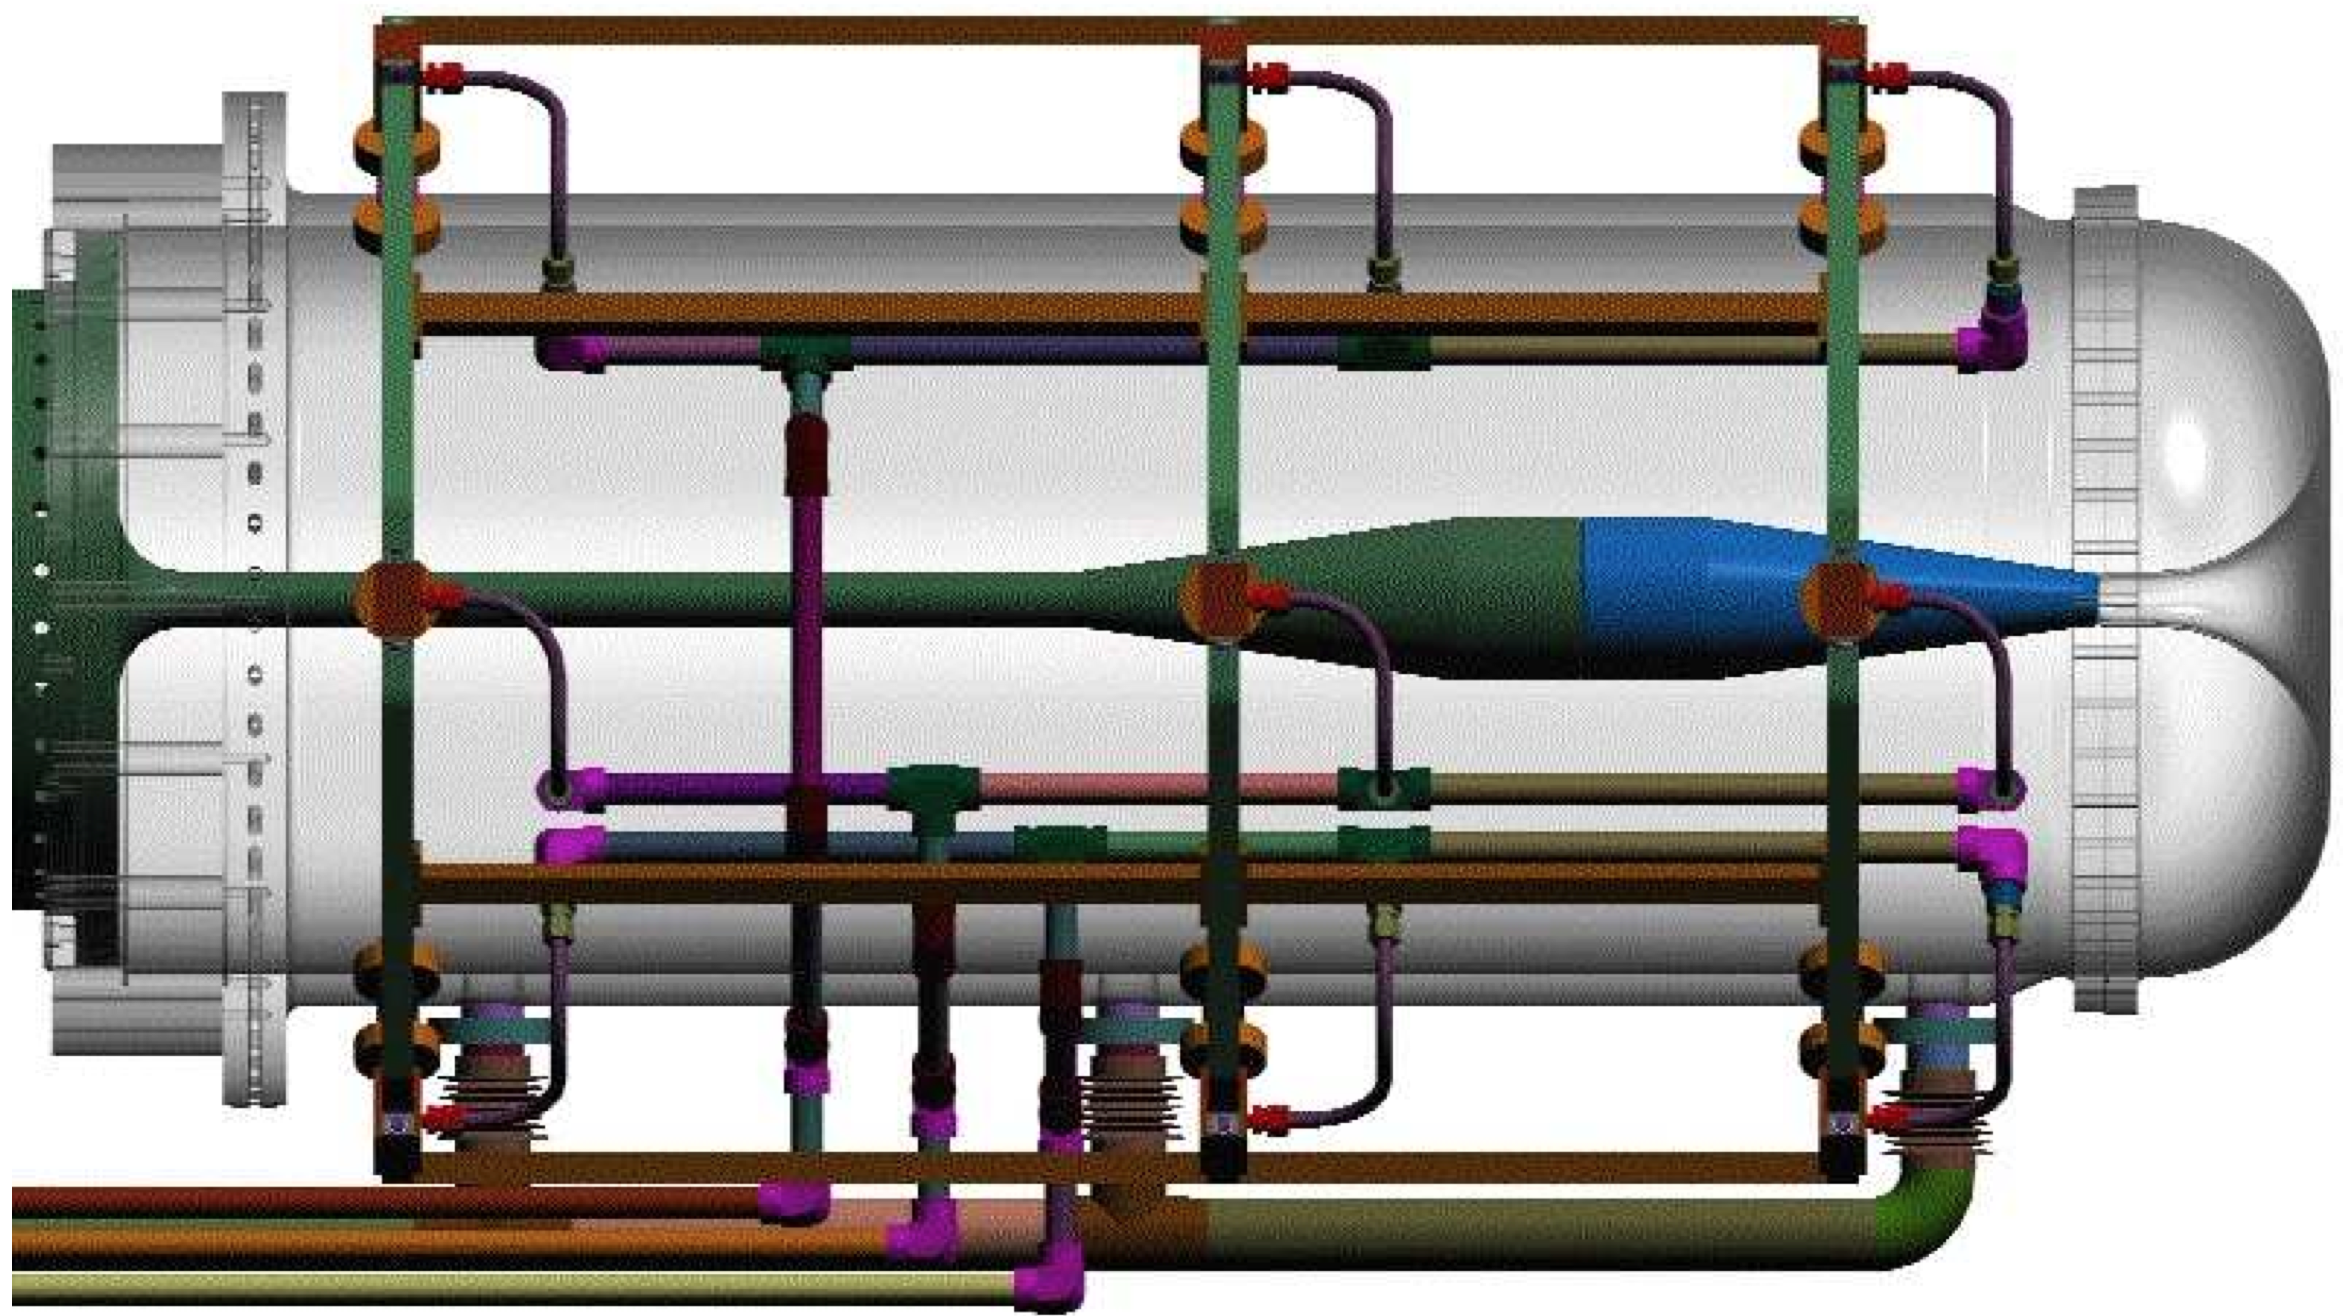
\includegraphics[width=0.7\textwidth]{Figures/BNB_horn_schematic.png} \\
\caption{\textit{The BNB focusing horn system. The gray outer conductor is drawn transparent for visualization purposes. The beryllium target lies within the central hollow tube axis. A current flows along the inner conductor, returning along the outer conductor.}}\label{BNB_horn_schematic}
\end{figure}

Downstream of the horn is a concrete collimator (214 cm long, between 30 cm and 35.5 cm in radius) which absorbs particles that would not otherwise contribute to the neutrino flux. Following the collimator is a 45 meter long (1 meter radius) air-filled cylindrical decay region, ending in a beam-stop made of steel and concrete which contains an array of gas proportional counters to detect muons penetrating the beam-stop. Also about half way through the length of the decay region is an absorber consisting of ten removable steel plates for systematic studies, which were not used in the analyses described in this thesis. A schematic depicting the proton beam interacting with the beryllium target within the focusing horn is shown in Figure \ref{BNB_numode_fig}.

\begin{figure}[ht!]
\centering
	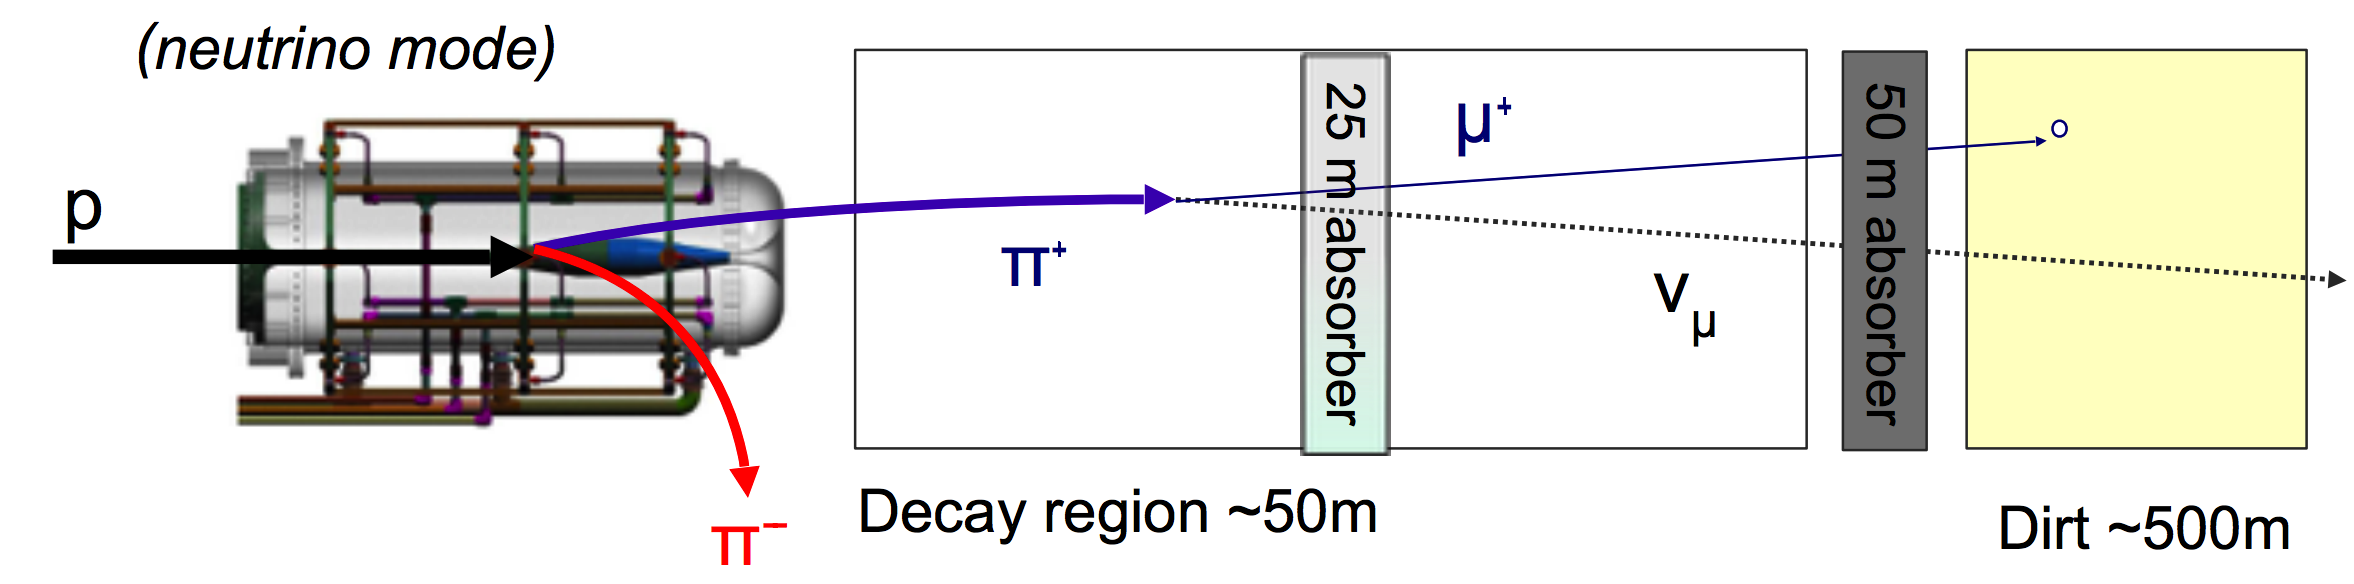
\includegraphics[width=1.0\textwidth]{Figures/BNB_numode_fig.png} \\
\caption{\textit{A cartoon diagram of the incident 8.89 GeV/c proton beam (from the left) colliding with the beryllium target within the focusing horn. Shown is the current configuration for the horn referred to as ``neutrino mode'' in which positive charged secondaries are focused into the decay region. The 25 m absorber drawn is removable, and was not used for the analyses described in this thesis.}}\label{BNB_numode_fig}
\end{figure}



\section{Monte Carlo Neutrino Flux Prediction}\label{beam_flux_descript_section}

The neutrino flux through MicroBooNE is determined using a Geant4~\cite{GEANT4source} Monte Carlo simulation of the beam-line, focusing horn, and decay region. The beam-line geometry modeled in Geant4 includes the position and material composition of all components of the BNB, through which the primary protons and all other particles propagate. The primary protons are simulated with the expected beam optics properties upstream of the target. The primary p-BE interactions are simulated using custom tables for the production of outgoing particles including protons, neutrons, $\pi^\pm$, $K^\pm$, and $K^0$ created from production models based on external data. The reason custom tables are used is that the variation in Geant4 hadron-production models is large.\\

The custom physics model using external data to simulate the production of secondary mesons in the primary p-Be interactions is described in detail in Ref ~\cite{MBFluxPaper} but will be summarized here. The custom tables describe the double differential cross section for the production of each secondary species as a function of the proton transverse and longitudinal momentum components. Existing pion and kaon production data from the HARP ~\cite{HARPgary8}, E910 ~\cite{E910source}, and several other production experiments are used in many of the Sanford and Wang parameterization fits in the parameter space relevant to MicroBooNE ~\cite{FEYNMANgary6}. The fitting parametrization is described with 9 Sanford-Wang model parameters ($c_1$ to $c_9$):
\begin{equation}\label{SWparamequation}
\frac{d^2\sigma}{dpd\Omega} = c_1p^{c_2}\left(1-\frac{p}{p_B-c_9}\right)\exp\left[-c_3\frac{p^{c_4}}{p_B^{c_5}}-c_6\theta(p-c_7p_B\cos^{c_8}\theta)\right]
\end{equation} 
where $p$ and $\theta$ are the momentum and angle of the outgoing secondary mesons.\\

Since no measurements for $K^+$ production exist at the 8.89 GeV/c BNB primary proton momentum, the Feynman scaling hypothesis is used to extrapolate from $K^+$ production measurements at different primary proton momenta. The Feynman scaling model function depends only on the transverse proton momentum $p_T$ and the Feynman scaling factor $x_F$, which is the ratio of the longitudinal momentum, $p_L^{CM}$, to the maximum longitudinal momentum, $p_L^{CM(max)}$,
\begin{equation}\label{feynmanscalingequation}
x_F = \frac{p_L^{CM}}{p_L^{CM(max)}}.
\end{equation}
According to the Feynman scaling model, the invariant cross section can be written in terms of seven parameters ($c_1$ to $c_7$) as
\begin{equation}\label{feynmanscaling_crosssec}
E\frac{d^3\sigma}{dp^3} = c_1\exp[-c_2p_T-c_3|x_F|^{c_4}-c_5p_T^2-c_7|p_T\dot x_F|^{c_6}]
\end{equation}
While this parameterization represents the measurements well, the uncertainties used in analyses by MiniBooNE were initially inflated by a factor of four to account for some inconsistencies within the production data. A more recent measurement by the SciBooNE collaboration indirectly measured the $K^+$ production in the BNB to drastically reduce this uncertainty ~\cite{gary_kaon_production_paper}.\\

With the outgoing particle production simulated, these particles are propagated with Geant4 taking into account energy loss and electromagnetic and hadronic processes, including the impact of the horn magnetic field on the kinematics of those particles. A custom decay model is used outside of the Geant4 framework to simulate the decay processes that result in neutrinos, which includes the latest branching fraction measurements and simulates polarization effects and kinematic distributions resulting from decay form factors. A number of techniques to enhance the statistical precision of the flux are employed~\cite{MBFluxPaper}.\\

The systematic uncertainties in the neutrino flux production come from several sources, which are summarized in Table \ref{flux_sys_uncerts}. The dominant uncertainty is that from particle production. By varying parameters in all of these systematic sources, a systematic error envelope is calculated for the final neutrino flux through the MicroBooNE detector. Figure \ref{UB_flux_fig} shows the $\nu_\mu$, $\overline{\nu}_\mu$, $\nu_e$, and $\overline{\nu}_e$ flux at the MicroBooNE detector. The red bars show the systematic error envelope, which includes all errors except those for proton delivery, which is a flat normalization error. Table \ref{UB_flux_sys_table} summarizes the systematic errors for the integrated flux.

\begin{table}
\begin{tabular}{ |p{4cm}|p{10cm}|  }
 \hline
 \multicolumn{2}{|c|}{MicroBooNE BNB Flux Systematics} \\
 \hline
 Source & Description \\
 \hline \hline
 Proton delivery & Counting the number of protons arriving on the beryllium target. \\\hline
 Particle production & Rate and shape of secondary particles produced in p-Be interactions. \\\hline
 Hadronic interactions & The rate of hadronic interactions in target or horn. \\\hline
 Horn magnetic field & Magnetic field to focus the outgoing charged mesons from p-Be interactions. \\\hline
 Beam-line geometry & Possible misalignments or displacements of beam-line components from their expected orientations. \\\hline
 Horn skin depth & Non-uniformity of current in the inner conductor of horn. \\\hline 
 \hline
\end{tabular}
\caption{\textit{A summary of the systematic uncertainties included in the MicroBooNE flux prediction. The dominant uncertainty is that from particle production.}}\label{flux_sys_uncerts}
\end{table}


\begin{figure}[ht!]
\centering
	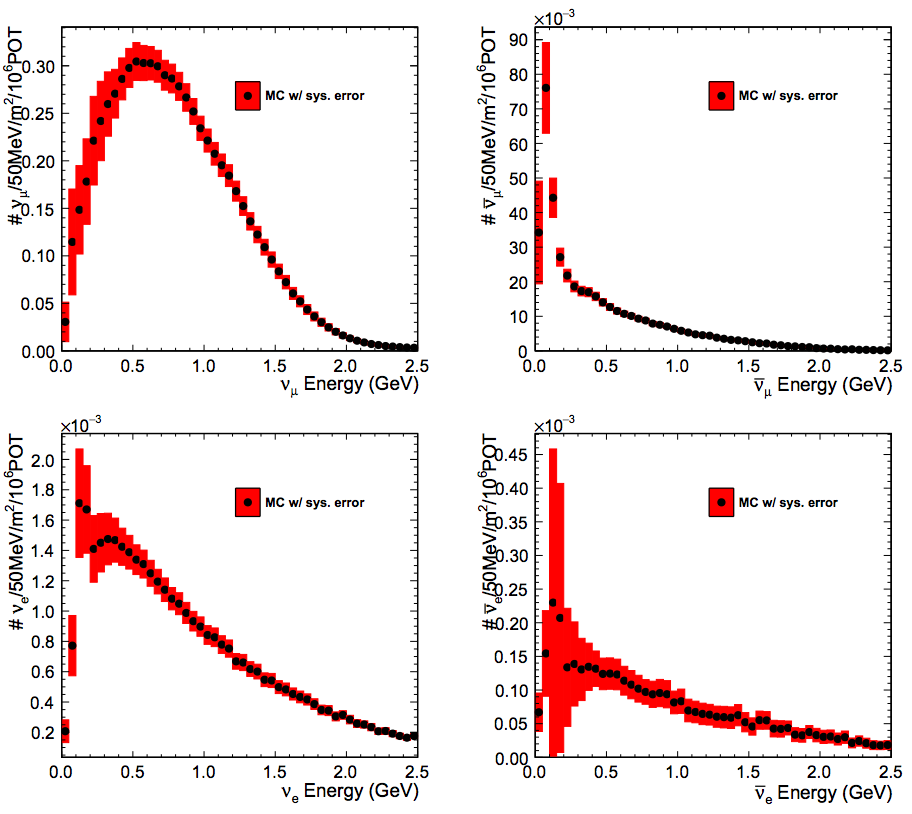
\includegraphics[width=1.0\textwidth]{Figures/UB_flux_fig.png} \\
\caption{\textit{Neutrino flux prediction (black dots) with systematic error bars (red envelope) excluding proton delivery systematics which results in a flat normalization correction.}}\label{UB_flux_fig}
\end{figure}

\begin{table}
\centering
\begin{tabular}{ |p{3 cm}|p{1.2 cm}|p{1.2 cm}|p{1.2 cm}|p{1.2 cm}|   }

 \hline
  & $\nu_\mu$ & $\overline{\nu}_\mu$ & $\nu_e$ & $\overline{\nu}_e$ \\
 \hline 
 POT Delivery & 2.00\% & 2.00\% & 2.00\% & 2.00\% \\
 $\pi^+$ & 5.80\% & 0.46\% & 4.62\% & 2.66\% \\
 $\pi^-$ & 0.01\% & 7.51\% & 0.28\% & 3.20\% \\
 $K^+$ & 0.38\% & 0.13\% & 5.19\% & 2.67\% \\
 $K^-$ & 0.01\% & 0.35\% & 0.28\% & 3.92\% \\
 $K^0_L$ & 0.03\% & 0.27\% & 2.36\% & 22.59\% \\
 Other & 5.78\% & 6.09\% & 3.60\% & 7.61\% \\\hline
 Total & 8.44\% & 9.89\% & 8.43\% & 24.74\% \\\hline
 \hline
\end{tabular}
\caption{\textit{A summary of the systematic errors for the integrated flux, mostly from particle production. ``Other'' includes hadronic interactions, horn current uncertainty, and skin effect.}}\label{UB_flux_sys_table}
\end{table}
